\chapter{Related Work}

%Propose only using PGExplainer for Node classification task.\bigskip
Yuan et al. \cite{yuan2022explainability} performed an extensive taxonomic survey on explainability in graph neural networks. We use this survey to discuss different approaches and motivate the selection of the PGExplainer in Section \ref{sec:gnn_explainability}. The authors note that the PGExplainer "is not performing as promising as its original reported results" \cite{yuan2022explainability}. Nevertheless, we evaluate the explainer model with regard to its applicability in the inductive setting. In Section \ref{sec:Explainer_Models} we briefly introduce important work related to the PGExplainer, as well as the model itself, since it is the core of our work. Lastly, we refer to NeuroSAT, which we use as a downstream model for the PGExplainer to generate explanations for its predictions on the SAT problem in Section \ref{sec:Downstream_Models}.

\section{Explainability in GNNs}
\label{sec:gnn_explainability}

Methods in DL have seen growth in performance in many tasks of artificial intelligence, including GNNs, since graphs are able to capture real-world data such as social networks or chemical molecules \cite{ying2018graph}, \cite{ma2021deep}. However, the interpretability of these models is often limited due to their black-box design \cite{noor2024survey}. Explainability methods aim to bypass this limitation by designing post-hoc techniques that provide insights into the decision-making process in the form of explanations. Such human-intelligible explanations are crucial for deploying models in real-world applications, especially when applied in interdisciplinary fields \cite{ribeiro2016should}.

There exist several different approaches for explaining predictions of deep graph models, that can be categorized into instance-level methods and model-level methods (see Yuan et al.  \cite{yuan2022explainability}). Instance-level methods aim to explain each input-graph by identifying important input features for its prediction, leading to input-dependent explanations. These can further be grouped by their importance score calculation into four branches. Gradients/feature-based methods use gradients as approximations of importance scores. Sensitivity Analysis \cite{baldassarre2019explainability} is an example that directly uses squared values of gradients as importance scores of input features. This enables the scores to be calculated directly with back-propagation.

Perturbation-based approaches like GNNExplainer \cite{ying2019gnnexplainer} and PGExplainer \cite{luo2020parameterized} study the variation of the output with regard to different input perturbations. The intuition behind this is that when input information crucial to the prediction is kept, the new prediction should roughly align with the prediction from the original input. PGExplainer aims to improve the GNNExplainer by providing a way of generating explanations with a global understanding of the GNN, significantly improving the computational cost. Another approach is SubgraphX \cite{yuan2021explainability}, which utilizes Monte Carlo Tree search to generate subgraph-level explanations. This does however entail a higher computational cost. 

Surrogate methods for deep graph models are inspired by surrogate methods for image data, that rely on neighboring areas of an input. Since graph data is concrete and contains topological information it is difficult to define the neighboring regions of an input graph. The idea is to obtain a local dataset containing neighboring data objects and predictions and fitting a simple, interpretable surrogate model to learn the local dataset. The explanations of the surrogate model are then regarded as the explanations of the original model. GraphLime \cite{huang2022graphlime} is an example that considers the $N$-hop neighboring nodes of a target node as the local dataset, where $N$ may be the number of GNN-layers. The weighted features of a non-linear surrogate model are then regarded as explanations. However, this method only explains node features, rather than the graph structure.

Decomposition methods, also motivated by success in the image domain, aim to measure input feature importance by decomposing the prediction into several terms, regarded as feature dependant importance score. Approaches for deep graph neural networks, like Layer-wise Relevance Propagation \cite{baldassarre2019explainability}, decompose the output prediction score to node importance scores. The decomposition rule is based on hidden features and weights, only enabling the study of node importance rather than graph structures.

Model-level methods, on the other hand, aim to explain GNNS without considering specific inputs, leading to input-independent, high-level explanations.


To fully trust the explanations provided by an explainer model, they must satisfy certain criteria, since there often is a mismatch between the optimizable metrics like accuracy and the actual metric of interest, which may not be measurable (see Ribeiro et al. \cite{ribeiro2016should}). First and foremost, an explanation should be \textbf{interpretable} and therefore provide qualitative, human-understandable interpretations, that also consider the possibility of limited user knowledge. Additionally, \textbf{local fidelity} asserts that explanations should be faithful in a local context and consider the models' behavior in the vicinity of predicted instances. Explainers that treat the model to be explained as a black-box are \textbf{model-agnostic} and should therefore be able to explain any model. Lastly, a \textbf{global perspective} is needed to explain a model fully, allowing us to take sample explanations of individual predictions that serve as representation of the model.

TODO: Claims to satisfy?
Since the perturbation-based PGExplainer \cite{luo2020parameterized} claims to satisfy all the criteria, while also maintaining reasonable computational cost, we select this model for the course of this study. It is furthermore able to generate explanations in an inductive setting, which we aim to do in \ref{}.

The general pipeline for different perturbation based approaches (see Figure \ref{fig:perturbation_pipeline}) can be described as follows: First, the important features from the input graph are converted into a mask by our generation algorithm, depending on the explanation task at hand. These masks are applied to the input graph to highlight said features. Lastly, the masked graph is fed into the trained GNN to evaluate the mask. The mask generation algorithm is updated according to the similarity of the predictions on the original and masked graphs. 

These different approaches mostly differ in the specific mask generation algorithm, the type of mask used and the objective function. It is important to distinguish between soft masks, discrete masks and approximated discrete masks. Soft masks take continuous values between $[0,1]$ which enables the graph algorithm to be updated via backpropagation. A downside of soft masks is that they suffer from the "introduced evidence" problem (see Dabkowski et al. \cite{dabkowski2017real}). Any mask value that is non-zero or non-one may add new semantic meaning or noise to the input graph, since graph edges are by nature discrete. Discrete masks however always rely on non-differentiable operations, e.g. sampling. Thus, the approximated discrete masks utilize reparameterization tricks to avoid the "introduced evidence" problem while also enabling back-propagation. %TODO: Expand on reparameterization trick?

Explanations can on the one hand be evaluated by visualizing the graph and considering the "human-comprehensibility". Since this requires a ground truth, is prone to the subjective understanding and is usually performed for a few random samples, it is important to apply stable evaluation metrics. One relevant accuracy metric for synthetic datasets with ground truths is the Area Under the Receiver Operating Characteristic Curve (ROC-AUC) (see Richardson et al. \cite{RICHARDSON2024100994}). The Receiver Operating Characteristic (ROC) curve plots the False Positive Rate (FPR) on the x-axis against the True Positive Rate (TPR), across different classification thresholds. The area under the curve (AUC) is calculated for said curve, resulting in the ROC-AUC, also referred to as AUROC. It is important to note, that a value of $0.5$ equals random guessing, while a score of $1.0$ indicates perfect classification. TODO: Other metrics include fidelity, results of taxonomy propose only using PGExplainer for Node Classification as it achieves low fidelity on Graph tasks

TODO: figure of perturbation pipeline?
\begin{figure}
    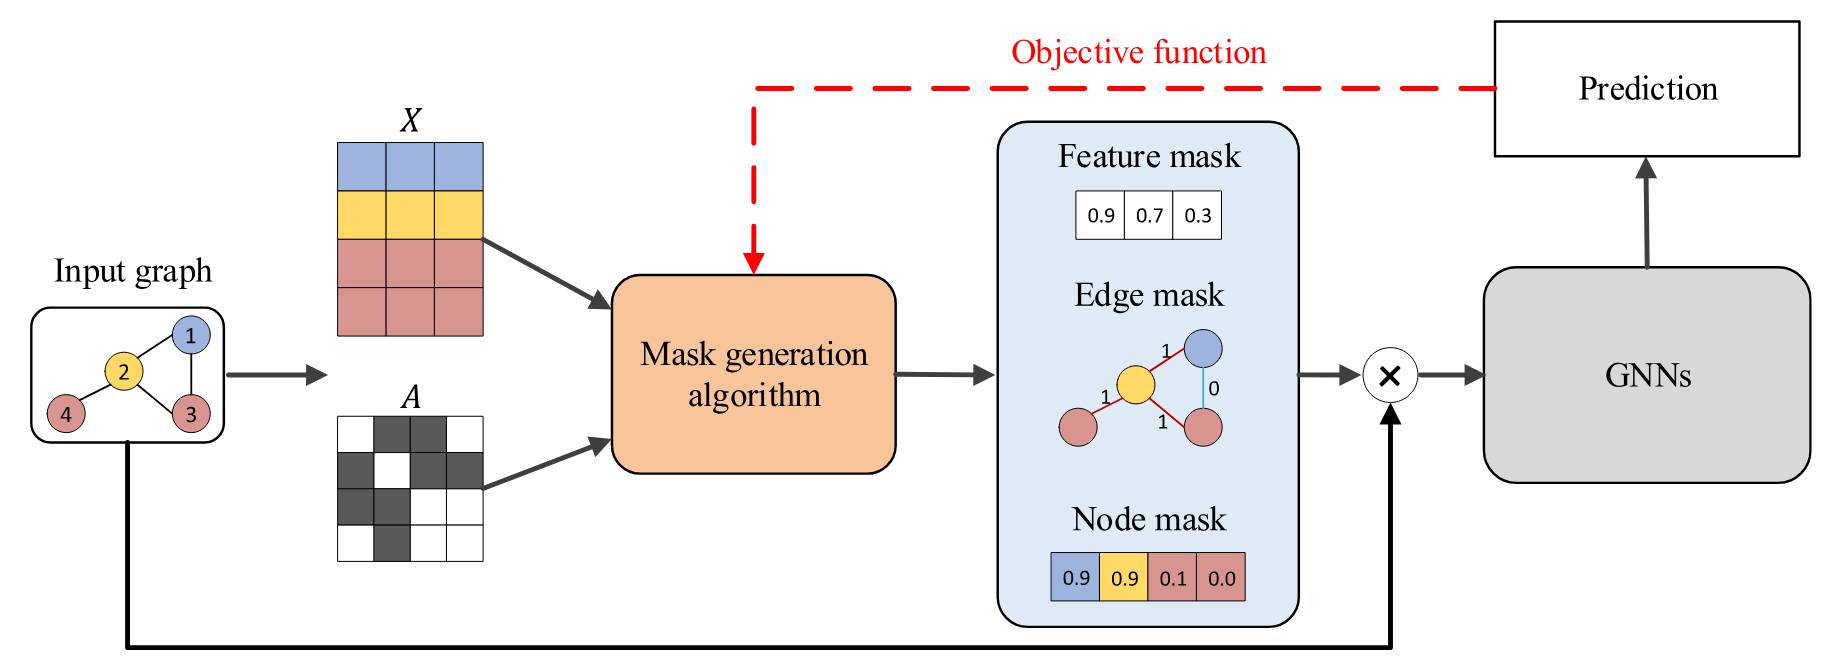
\includegraphics[width=\textwidth]{img/perturbation_pipeline.png}
    \caption{\small General pipeline of perturbation-based methods with a soft mask for node features, a discrete mask for edges, and an approximated discrete mask for nodes. The prediction of the GNN for the masked input graph is used in the objective function to train the generation algorithm and learn explanations. Reprinted from \cite{yuan2022explainability}.}
    \label{fig:perturbation_pipeline}
\end{figure}

\section{TODO: SECTION NAME Explainer Models}
\label{sec:Explainer_Models}

\textbf{GNNExplainer} \\
Ying et al. proposed the GNNExplainer \cite{ying2019gnnexplainer} - the first general, model-agnostic explainer for graph neural networks on any graph-based machine learning task. It is able to identify a concise subgraph structure and a subset of node features, that play a crucial role in the prediction of the underlying graph neural network. This is generally understood as an explanation. The work by Ying et al. serves as the main baseline for the PGExplainer, that seeks to improve its predecessor. Many concepts, experiments and specifications of PGExplainer were adapted from the GNNExplainer, which we seek to process in our work. \bigskip

\textbf{Parameterized Explainer for Graph Neural Networks} \\
The Parameterized Explainer for Graph Neural Networks (PGExplainer) by Lou et al. \cite{luo2020parameterized} is the main subject of our work. The idea of the framework is to collectively explain predictions of GNNs on a set of instance, while at the same time being able to generalize the explainer model to unexplained instances in an inductive setting. To achieve this, the method adapts a deep neural network to parameterize the generation process of explanations. %The method adopts a deep neural network to parameterize the generation process of explanations, thus allowing multiple instances to be explained collectively. Furthermore, it has better generalization ability and can explicitly be utilized in an inductive setting.

We reimplement the original work using PyTorch \cite{paszke2019pytorch} and PyTorch Geometric \cite{Fey/Lenssen/2019} instead of TensorFlow \cite{tensorflow2015-whitepaper}, while also emphasizing its application in an inductive setting, where test instances are unseen during training, as opposed to the original collective setting. A secondary study on the inductive performance was also performed by the authors, which we want to extend by applying it on a graph neural network with a slightly different architecture, testing whether the explainer proves to be model-agnostic. The goal of this thesis is to apply the explainer model to a deep learning approach for solving a bipartite graph problem - specifically, the boolean satisfiability problem - and generate proofs for the deep model's predictions. \bigskip

%This extension is motivated by the need for explainability methods that generalize across architectures (TODO: SOURCE FOR THIS).

\textbf{[Re] Parameterized Explainer for Graph Neural Network} \\
%We try own reimplementation that follows the original paper, as well as code and reimplementation for uncertainties + use a slightly different architecture in underlying GNN + Hyperparameter search of combination of parameters used in original and repication. Treated as additional baseline
Holdijk et al. \cite{holdijk2021re} performed a replication study on the PGExplainer that focuses on reimplementing the method in PyTorch, testing whether the claims with respect to the GNNExplainer hold and discussing whether the used evaluation method makes sense. They highlight a large discrepancy between the paper and codebase, making a replication that includes the evaluation method from the paper alone impossible. With help of the codebase, the authors are able to replicate the experiments and verify the main claims of the original paper. However, they express some concerns regarding the evaluation setup and note a large difference between the originally noted AUC scores and their results for most of the datasets. Additionally, they question the general approach for evaluating graph data with ground truths, as done in GNNExplainer and PGExplainer, which we will discuss in \ref{}. We use this work as an additional baseline for our approach, but note that the replication was also done in the collective setting. Therefore, the difference to our work lies mainly in the architecture used for the downstream model and the setting of the experiments.


\section{TODO: SECTION NAME Downstream Model}
\label{sec:Downstream_Models}

\textbf{NeuroSAT} \\
NeuroSAT by Selsam et al. \cite{selsam2018learning} is a machine learning approach for solving the boolean satisfiability problem using a message passing neural network. It is able to detect satisfying assignments, but lacks proofs of unsatisfiability. The authors performed a small study on the detection of unsat cores, revealing that NeuroUNSAT is able to detect UNSAT cores if the UNSAT problems contain a specific UNSAT core. However, this is expected to be due to the model memorizing the unsat cores, rather than generalizing to any unsat core. We want to test this by applying the PGExplainer in an inductive setting to the NeuroSAT model, and evaluate whether the generated explanations do align with unsat cores.